%Last edited 2026.02.21
% Evaluating the Hodgkin-Huxley model

\section{Hodgkin\&Huxley's empirical description\label{sec:Physiology-HodgkinHuxley}}


We admire the contribution of Hodgkin and Huxley,
and especially that they were wery critical concerning the validity ot their own quantized observations. They admitted that their model was not correct in some aspects. However,
their followers made their works the 'Holy Bible' of physiology,
with their really bright ideas and some wrong choices they made. In this section we summarize their 'model', given that the fallacies discussed in this chapter are the direct consequences of some mistakes in the model.

As we discuss in section~\ref{sec:Physics-Electricity}, the body's electric signals
were discovered early, the principles, notions and technical equipments have been elaborated.
Even, some meticulous measurements correctly interpreted some of its signals. 
The development of electronical technology enabled their systematic study 
in the beginning of the 50's. However, experimenters 
often forgot that "\textit{Under ideal
circumstances, the physical act of measuring a neurophysiological event
would have no effect on the electrical signal of interest. Unfortunately,
this is seldom the case in neurophysiology.}"~\cite{JohnstonWuNeurophysiology:1995}.
	

The first systematic attempt to describe the results of observations in terms of the well-known laws of electricity
 was published around 1952~\cite{HodgkinHuxley:1952}.
A collection of their (modernized) papers is available~\cite{CompanionGuideHodgkinHuxley:2022}.
They made a huge amount of \hypertarget{HHmeasurements}{meticulous measurements}
and wanted to help the science community with providing equations for practical applicability.
To speed up reaching that goal, they introduced \textit{empirical functions} 
and derived equations, which, not surprisingly, described the \textit{empirical observations} quite accurately. 
The importance of their work is best highlighted by that it inspired 
different disciplines for discussion. 

\quotationbox{
"although highly successful
in predicting and explaining many of the electric characteristics of the action
potential, the HH model, nevertheless cannot accommodate the various non-
electrical physical manifestations (mechanical, thermal and optical changes)
that accompany action potential propagation, and for which there is ample
experimental evidence.~\cite{NerveSignalAsWindow:2023}
}

A technical reason is described in~\cite{HodgkinMemoryBook:1992}:
"The fact that the whole process for calculation of a $4-5\ ms$ interval,
showing the initiation of and recovery following an action potential, could be accomplished in 8 hours is astonishing."
The must-be oversimplification does not belong to the core of the theory.
When using the recent computing systems, not necessarily the old oversimplified models should be coded.
One could also use modern, more compute intensive, and physically correct models.

\subsubsection{Model summary\label{sec:Physiology-HodgkinHuxleyModelSummary}}
\begin{figure}
\centering
	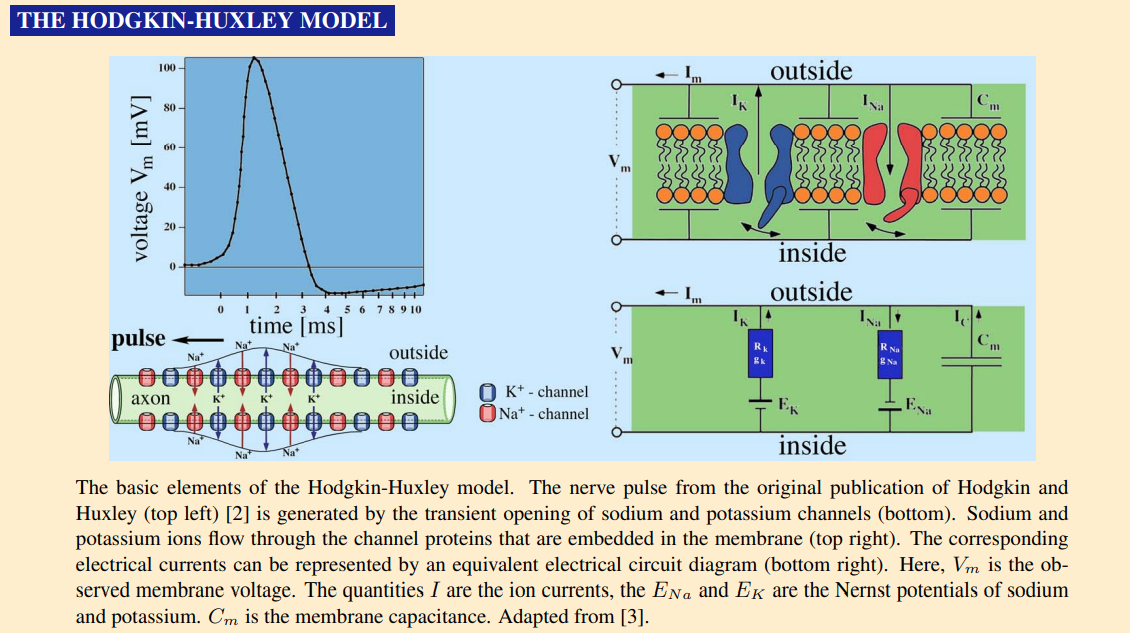
\includegraphics[width=\textwidth]
	{fig/HHModelHeimburg.png}
	\caption{The Hodgkin-Huxley model as reproduced by~\cite{HeimburgPhysikOfNerves:2009}}
	\label{fig:HHModelSummary}
\end{figure}


\subsubsection{Self-evaluation\label{sec:Physiology-HodgkinHuxleySelfEvaluation}}
In their brilliant publication~\cite{HodgkinHuxley:1952}, 
Hodgkin and Huxley evaluated their results "that our equations [must not be taken as] anything more than an empirical
description" and "the [partial] success of the
equations is no evidence in favour of the mechanism". 
When validating their observations,
they have found serious question marks: "a number of points were noted on which the calculated behaviour of our model
did not agree with the experimental results. We
shall now discuss the extent to which these discrepancies can be attributed to
known shortcomings in our equations."
"One was that the membrane capacity was assumed to
behave as a \textit{'perfect' condenser}, \dots the other was
that the equations governing the potassium conductance do not give as much
\textit{delay in the conductance rise} on depolarization as was observed in voltage clamps".
They did have the intuition that something was wrong and they correctly guessed its reason:
"it seems difficult to escape the conclusion that the changes
in ionic permeability depend on \textit{the movement of some component} of the
membrane \textit{which behaves as though it had a large charge}.\dots it is necessary to suppose
that \textit{there are more carriers and that they react or move more slowly} \dots \textit{there is no evidence from our
experiments of any current associated} with the change in sodium permeability, apart from the contribution of the sodium ion itself".

They emphasized that their work 
"must not be taken as evidence that their equations are anything more than an empirical description".
They made the first step of "a great journey into the unknown" and were very cautious by saying
that "the success of the equations is no evidence in
favour of the mechanism that they tentatively had in
mind when formulating them".

In his late work~\cite{HodgkinMemoryBook:1992}, Hodgkin evaluated the filtered experiences:
"We soon realized that \textit{the carrier model could not be made to fit certain results},
for example the nearly linear instantaneous current voltage relationship, and
that it had to be replaced by some kind of voltage-dependent gate. As soon as
we began to think about molecular mechanisms it became clear that
\textit{the electrical data would by themselves yield only very general information} about the class
of system likely to be involved. So we settled for the more pedestrian aim of
finding a simple set of mathematical equations which might plausibly represent
the movement of electrically charged gating particles."


\subsubsection{Nobel-laudation\label{sec:Physiology-HodgkinHuxleyNobel}}

Unfortunately, they also attempted to understand which physical processes happen in the membrane,
but they concluded with the feeling that "\textit{the interpretation given is unlikely to provide a correct picture of the membrane}."
Despite their explicite warning, that "the success of the equations is no evidence in
favour of the mechanism that we tentatively had in
mind when formulating them". 
Despite, they received the Nobel-prise "for their discoveries concerning the
\textbf{ionic mechanisms} involved in excitation and inhibition in the peripheral and central portions of the nerve".
As the philosphical approach to their work discusses, "One could dismiss this curious passage as scientific modesty
if it were not for the fact
that Hodgkin and Huxley argue for their conclusions."~\cite{MechanisticModelHodgkinHuxleyCraver:2006}
The science community rushed to apply the equations, instead of validating them.
To compensate for the disagreements with the experimental data, further ad-hoc
assumptions have been introduced, making their admittedly wrong picture even worse.

In the sense of philosophy, "there is a widely accepted distinction between
\textit{merely modeling a mechanism’s behavior} and \textit{explaining} it.
The equations
must be supplemented by a causal interpretation: one might, for example, agree by
convention that the effect variable is represented on the left, and the cause variables
are represented on the right, or one might add “these are not mere mathematical
relationships among variables but descriptions of causal relationships in which this
variable is a cause and this other is an effect,” and not vice versa",
for more details see~\cite{MechanisticModelHodgkinHuxleyCraver:2006,Mechanistic_HodgkinHuxley_2008}.
The lack of causality is one reasons why
HH have had the feeling they missed the correct picture of the membrane.
The other reason is that some fine details of their oversimplified picture was not accurate,
althought the additional (and arbitrary) ad-hoc assumptions have hidden the disagreements.
The followers have "fitted elephants"~\cite{FittingElephants:2021} by adding many more ad-hoc effects with too many parameters.

\subsection{Measurement science\label{sec:Physiology-HHPhilosophy}}

As highlighted in ~\cite{MechanisticModelHodgkinHuxleyCraver:2006}, the performed a very meticulous analysis
and characterized the time-course of the action potential phe
nomenally terms of different features (the concise listing taken from~\cite{MechanisticModelHodgkinHuxleyCraver:2006})

\begin{itemize}
\item the form, amplitude, and threshold of an action potential;
\item the form, amplitude, and velocity of a propagated action potential;
\item the form and amplitude of the resistance changes during an action potential;
\item the total movement of ions during an action potential;
\item the threshold and response during the refractory period;
\item the existence and form of subthreshold responses;
\item the production of action potentials after sustained current injection (that is,
anodal break);
\item the subthreshold oscillations seen in the axons of cephalopods
\end{itemize}


"A measurement can be precise without being accurate."\cite{JohnstonWuNeurophysiology:1995} \textit{Accuracy means characterizing 
the true measurable quantity.} In this sense, their measurement is precise but not accurate: they measured precisely wrong quantities, which, unfortunately, can be made and thought sufficiently resemblant to the real ones. 

\subsection{Mathematics\label{Physiology-HHMathematics}}
"These equations and the methods that arose from this combination of modeling and
experiments have since formed the basis for every subsequent model for active cells.
The Hodgkin-Huxley model and a host of simplified equations  derived from
them have inspired the development of \textit{new and beautiful mathematics}." \cite{MathNeuroscience:2010}.


\subsection{Physics\label{Physiology-HHPhysics}}

"A. L. Hodgkin and A. F. Huxley published what was to become known as the
model of the action potential. This model would subsequently be considered a cornerstone of
electrophysiology and neuroscience, since it concerned the ionic mechanisms involved in the
operation of the nerve cell membrane."~\cite{PhysicsForHodgkinHuxley:2024}




\subsubsection{Neglecting Coulomb's Law\label{Physiology-HHNeglectingCoulomb}}

\index{Coulomb's law}

\subsection{Driving force\label{sec:Physiology-HHDrivingForce}}



As we discuss in section~\ref{Physics-OscillatorIntegrator}, HH introduced 
by their Eq.~(1) (reproduced by us as Eq.~(\ref{eq:OutputHH}))
the basic decription of \textit{the membrane current \textbf{during a voltage clamp}} with that 
"the justification for this equation is that it is the simplest which can be used
and that it gives values for the membrane capacity which are independent of
the magnitude or sign of $V$ and are \textit{little affected by the time course of $V$}".
(It is again a reversed approach: the capacity, per definitionem, means the ability to store charge
and is one of the attributes of the medium instead of the electric characteristic
of the tested circuit. For the case of \hyperlink{voltage-clamping}{clamping}, it is an approximation
that the temporal course of the clamping voltage
is kept constant, the current remains constant.  
As we discuss in section~\ref{sec:Physiology-NeuralCurrentsPATCHING},
in the case of a constant current where $I=\frac{dQ}{dt}$,  the voltage increase $dV$
on the capacity $C$ of the membrane is $\frac{dQ}{C}=\frac{I*dt}{C}$,
so we can derive the "driving force" (compare it to Eq.~(\ref{eq:Nernst-dVdt}))
as they interpreted it
%
\[\frac{d}{dt} V=\frac{I}{C}\label{eq:Physiology-HHDrivingForce}\]
%
The direct \textit{constant} current input $\frac{d}{dt} V_{PATCH}$
to the neuron cell body is a simple constant current that causes a constant membrane's voltage derivative contribution.
That is, if one checks the dependence of the output voltage on $\frac{d}{dt} V$ and $I$, in the presence of a constant $C$,
one observes the same dependence.
However, the currents are not necessarily constant.



